\documentclass[a4paper,12pt,openany]{report}

\usepackage{titling}
\usepackage[margin=0.75in,headsep=0.5in,footskip=0.5in]{geometry}
\usepackage{graphicx}
\usepackage{float}

\usepackage{enumitem}
\usepackage{placeins}

\setlist{nosep}

%\usepackage{parskip}

\setlength{\parindent}{0pt} % Remove Paragraph indenting
\setlength{\parskip}{10pt}

\renewcommand\thesection{\arabic{section}} % Remove Chapter Numbers

\newcommand{\subtitle}[1]{
	\posttitle{
		\par\end{center}
		\begin{center}\large#1\end{center}
		\vskip0.5em
	}
}

\newcommand{\coverphoto}[2]{
	\postdate{
		\par\end{center}
		\begin{center}
			\includegraphics[width=15cm]{#1}
		\end{center}
	}
}

% document

\begin{document}

% Title Page

\title{Swimming Pool Automated Checking System}
\subtitle{CITS4401 Software Requirements and Design - Practical Assignment}
\author{Mitchell Pomery (21130887)}
\coverphoto{images/the_general_problem}{XKCD 974}
\maketitle
\clearpage

\setcounter{tocdepth}{1}
\tableofcontents

\section{Introduction}

\par
The Swimming Pool Automated Checking System (SPACS) helps to keep track of and assist in the upkeep of private swimming pools. This document outlines the design of the SPACS system and is intended to be used as a reference guide by anyone involved in the creation the SPACS system.

\subsection{Terms}
\par
Below are a list of terms and abbreviations used in this document and their definitions.

\begin{center}
\begin{tabular}{| l | p{13cm} |}
\hline
API & Application Programming Interface - A set of functions that allow the manipulation of the system through defined procedures. \\ \hline
PTU & Pool Testing Unit \\ \hline
SPACS & Swimming Pool Automated Checking System \\ \hline
\end{tabular}
\end{center}

% Introduce everyone to what the document will tell them
\clearpage

% Covers the functional modelling aprt of the assignment
\section{Use Case Diagrams}

\par
CITS4401 Software Requirements and Design - Practical Assignment.
CITS4401 Software Requirements and Design - Practical Assignment.
CITS4401 Software Requirements and Design - Practical Assignment.
CITS4401 Software Requirements and Design - Practical Assignment.
CITS4401 Software Requirements and Design - Practical Assignment.
CITS4401 Software Requirements and Design - Practical Assignment.
%\clearpage
% What objects will be programmed and what they do
% Only objects that hold data will appear here
\newcommand{\object}[3]{
\begin{tabular}[h!]{| p{7cm} |}
	\hline
	\begin{center}\textbf{#1}\end{center} \\ \hline
	\begin{mylist} #2 \end{mylist} \\ \hline
	\begin{mylist} #3 \end{mylist} \\ \hline

\end{tabular}
}

\newenvironment{mylist}{
	\begin{enumerate}[label=+]
}{
	\end{enumerate}
}

\section{Object Models}

\begin{figure}[h!]
\begin{center}
	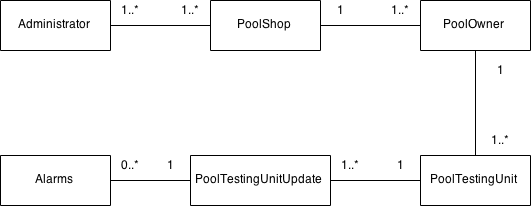
\includegraphics[width=15cm]{images/ObjectRelations}
	\caption{relationships between the main classes in the system}
\end{center}
\end{figure}

\par
There can be multiple administrators in the SPACS system that manage all the PoolShopAdmin. Each PoolOwner can only be registered at one PoolShopAdmin, and each PoolTestingUnit can only be linked to one PoolOwner. The Administrator, PoolShopAdmin and PoolOwner objects all contain information about a single person.
\par
The above figure shows the basics of how the different objects interact, and not the helper classes that ensure these links are done correctly. More information on how these classes interact can be found below.

\subsection{Objects}
\subsubsection{User}
\par
User is the class that all users of the system will fall under. It ensures a minimum amount of information is collected about each user and will implement all the basic instructions needed for interacting with the objects. The level property allows the user object to do this. Authentication information is stored in the Authentication object to minimize the ability to leak sensitive information, such as passwords from it.

\object{User(object)}
{
	\item id
	\item title
	\item name
	\item address 
	\item email\_address
	\item phone\_number
	\item mobile\_number
	\item level
}
{
	\item
}

\object{Authentication(object)}
{
	\item id
	\item username
	\item password
}
{
	\item
}

\subsubsection{Administrator, PoolShop and PoolOwner}
\par
These are all extensions of the User object and will implement any extra methods that they do not inherit. Pythonic code doesn't use setter and getter functions, but still allows the properties to have validation on them.

\object{Administrator(User)}
{
	\item 
}
{
	\item
}

\object{PoolShop(User)}
{
	\item pool\_owners
}
{
	\item 
}

\object{PoolOwner(User)}
{
	\item pool\_testing\_units
}
{
	\item
}

\subsubsection{ShopOwnerLink}
\par
ShopOwnerLink stores the link between a PoolShopAdmin and a PoolOwner, ensuring that  a PoolShopAdmin can only see pools that they manage.

\object{ShopOwnerLink(object)}
{
	\item pool\_shop\_admin\_id
	\item pool\_owner\_id
}
{
	\item
}

\subsubsection{PoolTestingUnit}
\par
Pool Testing Units are mostly passive users of the system and have the sole role of providing information to the system. They are closely linked to their PoolOwner. Again, due to the way python works this object should have no methods.

\object{PoolTestingUnit(object)}
{
	\item ptu\_id
	\item owner\_id
	\item length
	\item width
	\item depth
	\item volume
	\item above\_ground
	\item material
						
}
{
	\item
}

\subsubsection{PoolTestingUnitUpdate}
\par
PoolTestingUnitUpdate objects store all the information from the records that the pool testing units send.

\object{PoolTestingUnitUpdate(object)}
{
	\item report\_id
	\item ptu\_id
	\item datetime
	\item pH
	\item chlorine\_level
	\item chlorinator\_status
	\item total\_alkalinity
	\item temperature
	\item water\_hardness
	\item water\_level
	\item datetime\_last\_filter
	\item alarms
}
{
	\item
}

\subsubsection{Alarm}
\par
Alarm objects store alarms set off when a PoolTestingUnit sends a PoolTestingUnitUpdate.

\object{PoolTestingUnitUpdate(object)}
{
	\item alarm\_id
	\item report\_id
	\item reason
	\item value
	\item expected
}
{
	\item
}
%\clearpage
% 5 sequence diagrams for 5 use cases. Consistant with class diagrams
\section{Sequence Diagrams}

\par
The main functions that SPACS performs are all done at an API level. These diagrams show an abstraction of what the code does, starting with the actor as an end user of the system.

\subsection{regular\_update}
\par
A regular update starts when a PoolTestingUnit makes an API request against the WebServer. The WebServer forwards the request to the API layer which then populates a PT object which is stored in the database by a transaction bean.

\begin{figure}[!ht]
\begin{center}
	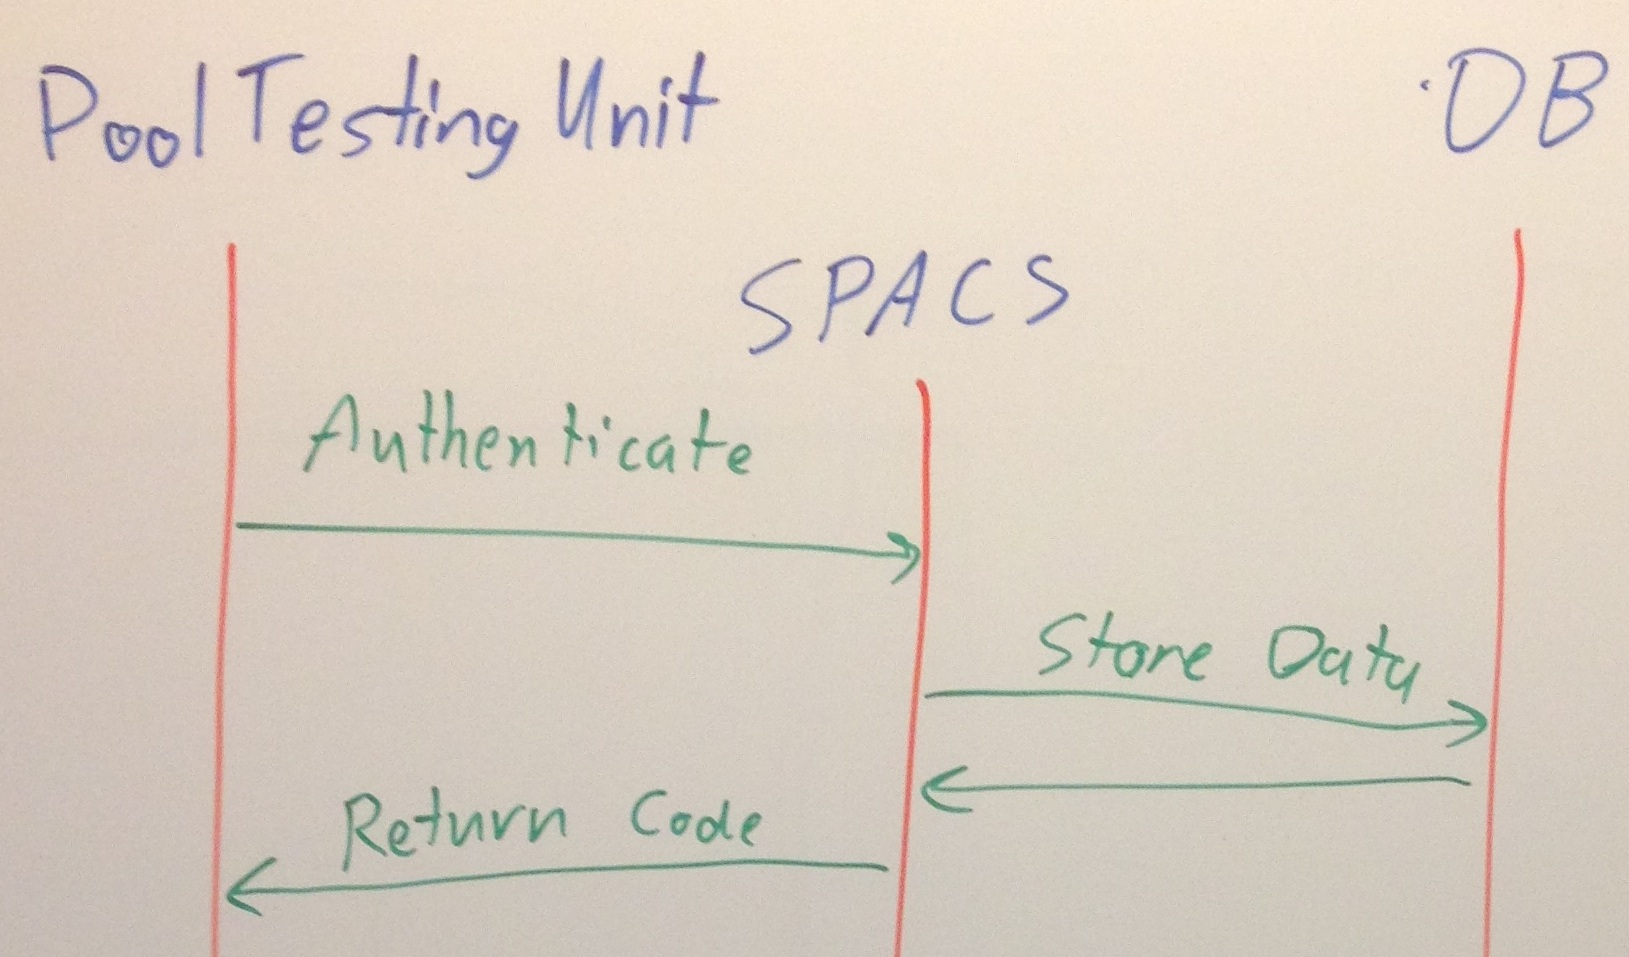
\includegraphics[width=14cm]{images/regular_update}
\end{center}
\end{figure}
\FloatBarrier

\subsection{urgent\_update}
\par
The urgent update differs to the regular update only by the PTUUpdate object sending off an email to the PoolOwner and PoolShopAdmin after the data is saved to the database.

\begin{figure}[!ht]
\begin{center}
	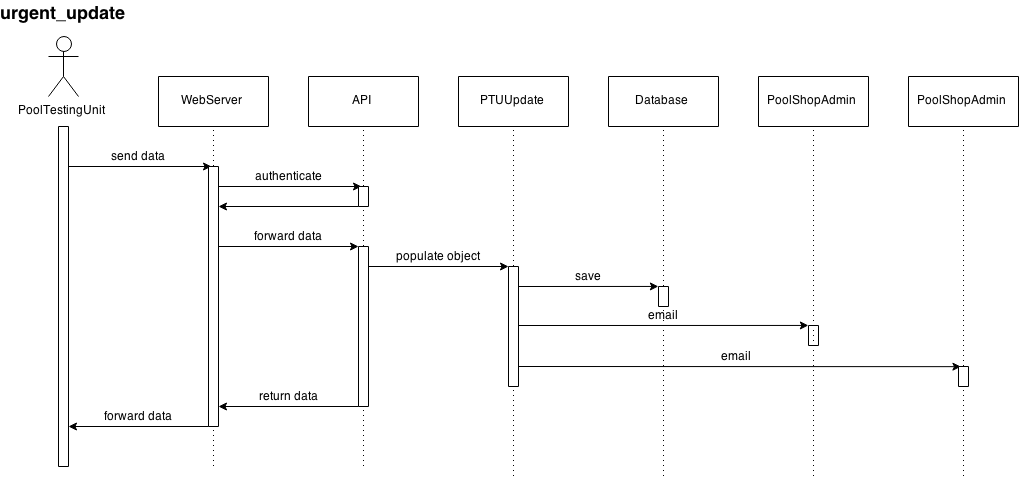
\includegraphics[width=14cm]{images/urgent_update}
\end{center}
\end{figure}
\FloatBarrier

\subsection{generate\_report}
\par
The ReportGenerator is started up by the Scheduler. It pulls in all the pools that need reports generated. These pools then pull in the information needed for the report. The ReportGenerator formats these nicely, then sends them off to the PoolOwner.

\begin{figure}[!ht]
\begin{center}
	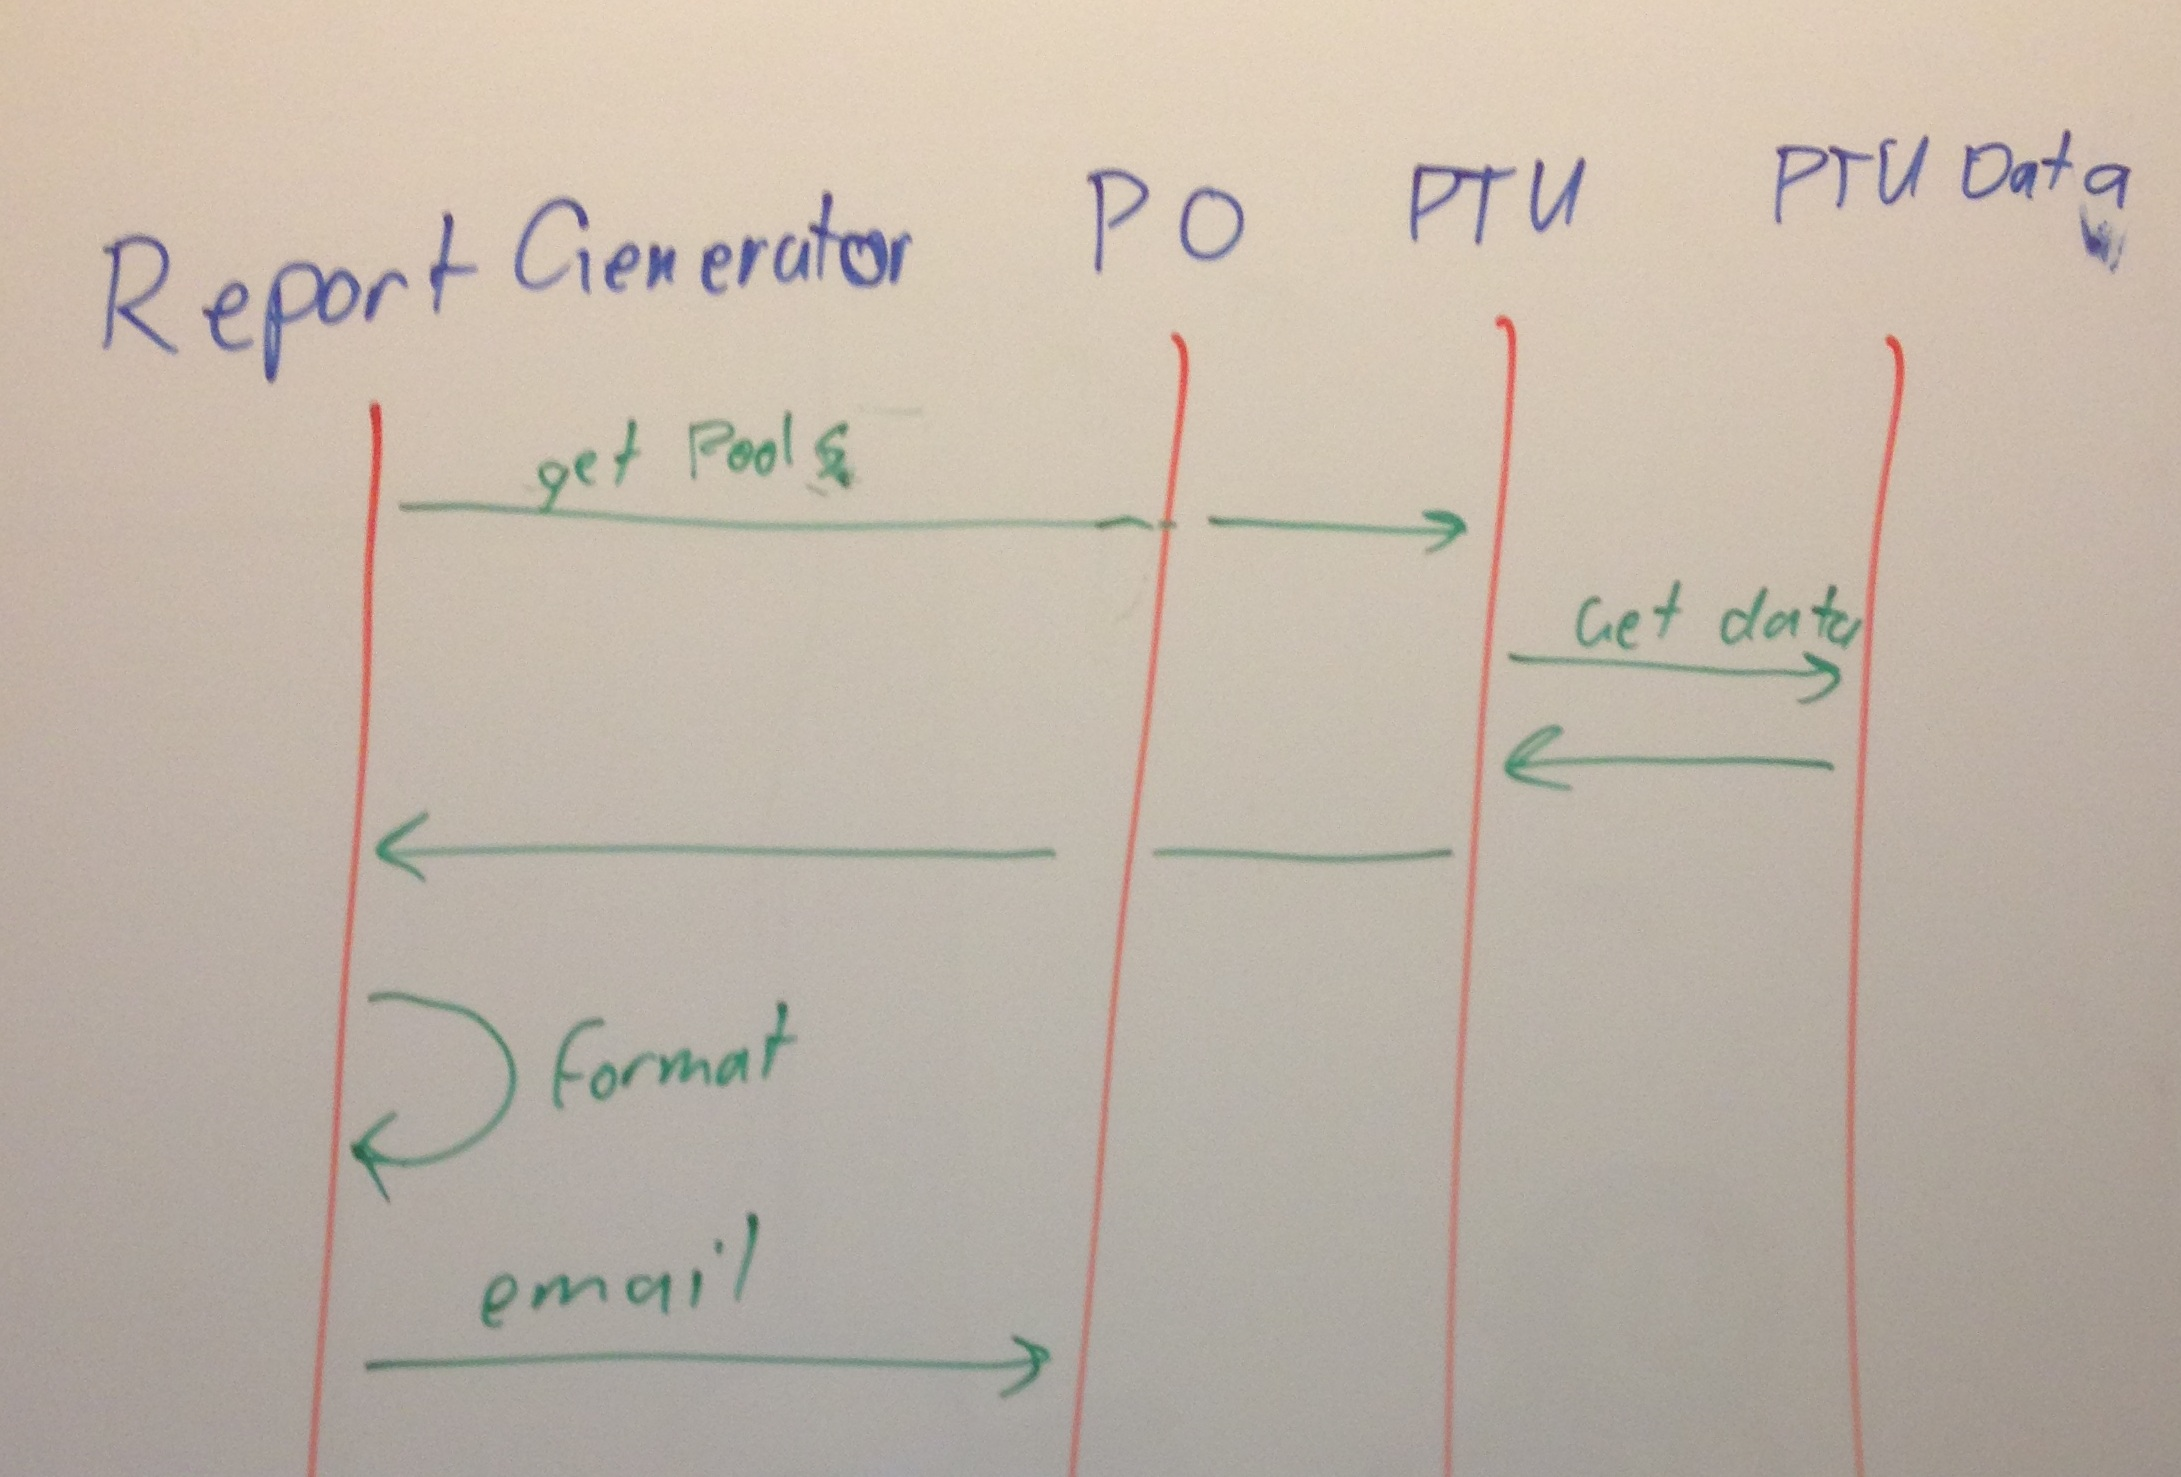
\includegraphics[width=14cm]{images/generate_report}
\end{center}
\end{figure}
\FloatBarrier

\subsection{edit\_pool\_shop\_admin}
\par
A PoolShopAdmin is edited by being sent the updated data via the web. This then gets parsed by the API which loads the PoolOwner out of the database. It's properties are then changed before being saved back to the database by the transaction bean. Information about the transaction is then returned to the user.

\begin{figure}[!ht]
\begin{center}
	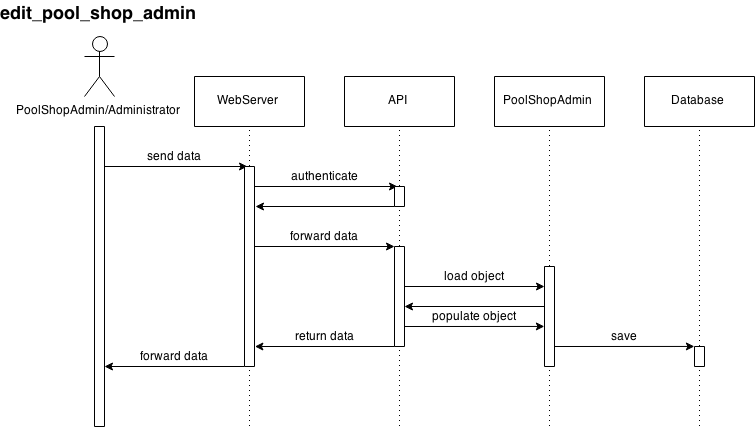
\includegraphics[width=14cm]{images/edit_pool_shop_admin}
\end{center}
\end{figure}
\FloatBarrier

\subsection{edit\_pool\_owner}
\par
Editing a PoolOwner is done in the same way as editing a PoolShopAdmin.

\begin{figure}[!ht]
\begin{center}
	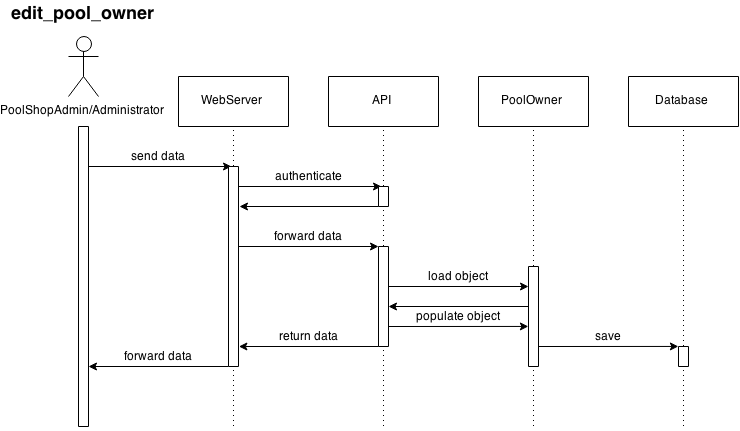
\includegraphics[width=14cm]{images/edit_pool_owner}
\end{center}
\end{figure}
\FloatBarrier
%\clearpage
% Not 100% sure what to do here
\section{Design Considerations}

\par
Decisions have been made to meet the quality requirements of the SPACS system listed below. These decisions aim to maximize each requirement while keeping the cost of development and running the system as low as possible.

\begin{enumerate}
	\item Performance
	\item Reliability
	\item Usability
	\item Portability
	\item Modifiability
	\item Future Requirements
\end{enumerate}

\subsection{Python}
\par
Python has been chosen as the implementation language over other object oriented languages such as Java due to it's lightweight footprint and portability. Python allows for rapid development and testing, making the system easy to modify. Well written Python code also has the advantage of being self documenting, meaning that is highly readable so less comments are required.

\par
Unlike other object oriented languages, Python is dynamically typed. This means that the types of each variable are not defined while developing, but rather at run time. Python is also an interpreted language, rather than a compiled one. This means that things such as type errors and non existent variables will only be found during run time. A full set of testing and good logging will minimize the risk of this causing issues while the system is in production.

\par
As python has been chosen, class and method names in this document are named according to the Python PEP 8 Style Guide.

\subsection{Statelessness}
\par
The application has been developed with scalability in mind meaning that all sessions should be stateless and information should not be managed by the program once it has finished with it. It will be possible to set up multiple instances of the server that are able to communicate with the same database. This will allow the application to scale in the event where the number of users increases past an individual servers load.

\par
Adding this scalability will require a load balancer to sit between the users and the server instances. The addition of the load balancer will also allow individual servers to be taken offline for updates or if there is an issue with a machine.

\subsection{API Based}
\par
Keeping the relationships between all the objects are kept as simple as possible minimizes the need for complex helper classes. As such, everything can be implemented as API calls made straight from the web application. This leads itself to making the application scalable, as as much of the work as possible is rendered at the client side.

\subsection{Transaction Beans}
\par
Transaction Beans are found in many enterprise Java applications and make modifying data in the database simple. They allow the object to be loaded from a database bean and will store any changes made to the object when completed. All object loading and saving will be done in the transaction beans, and the structure of in the code will mirror that of the database. As transaction beans centralize all database access any issues with the database and all logging of database requests will be dealt with here.

\subsection{Reliability}
\par
The SPACS system has been designed with reliability in mind. The ability to run multiple SPACS servers in a cluster minimizes the chance of downtime. It is also self contained and will restart itself after any fatal errors. Logging and email alerts also mean that an Administrator monitoring the system can easily find and diagnose problems.


%\clearpage
% Subsystems - what ones
\section{Subsystems}

\par
The SPACS system will be broken down into several subsystems.

\par
\begin{enumerate}
	\item Server
	\begin{enumerate}
		\item Website
		\item API
		\item Scheduler
	\end{enumerate}
	\item Database
\end{enumerate}

\par
The server subsystem is responsible for running the main portion of the program. It will start up all the subsystems below it according to a global configuration file. Any errors that the systems below it cause will be caught by the server and handled gracefully. It will also be responsible for making sure that any information from the systems below it are logged correctly.

\par
The website will be the main user interface and will be managed by the server. All connections to this will be stateless, meaning that several servers can be launched behind a load balancer and act together so that the system can be scaled up as the number of users increases if needed.

\par
The API will run on top of the Website and will be the only way that a user can interface with the database. This ensures that all the features the end user sees exist in one place.

\par
The scheduler will be responsible for running anything that is timing sensitive, such as report generation, or that may need to be retried, such as emailing. This ensures that all retry and timing logic will appear in only one location. Any thing that needs to be scheduled will be stored such that it can be accessed after the server has been restarted. Items that are scheduled will be responsible for setting their own timings and retry logic allowing the flexibility for them to react differently depending on their own outcomes.

\par
The database will be the one true source of all information for the system. It will not be managed by the server subsystem.


%\clearpage
% Statecharts for subsystems. Covers Dynamic Modelling
\section{State Charts}
%\clearpage
% Two that would be appropriate and why
\section{Design Pattern}

\par
CITS4401 Software Requirements and Design - Practical Assignment.
CITS4401 Software Requirements and Design - Practical Assignment.
CITS4401 Software Requirements and Design - Practical Assignment.
CITS4401 Software Requirements and Design - Practical Assignment.
CITS4401 Software Requirements and Design - Practical Assignment.
CITS4401 Software Requirements and Design - Practical Assignment.
\clearpage

%\begin{thebibliography}{20} 
%	\bibitem{ref_for_linking} Info
%\end{thebibliography} 


\end{document}
